\documentclass[border=0pt]{standalone}
\usepackage{tikz}
\usetikzlibrary{positioning,shapes,arrows.meta,patterns,calc}
\definecolor{garnet}{HTML}{73000A}
\definecolor{coral}{HTML}{CC2E40}
\definecolor{slate}{HTML}{466A9F}
\definecolor{teal}{HTML}{1F414D}
\definecolor{olive}{HTML}{65780B}
\definecolor{lime}{HTML}{CED318}
\definecolor{gold}{HTML}{A49137}
\begin{document}
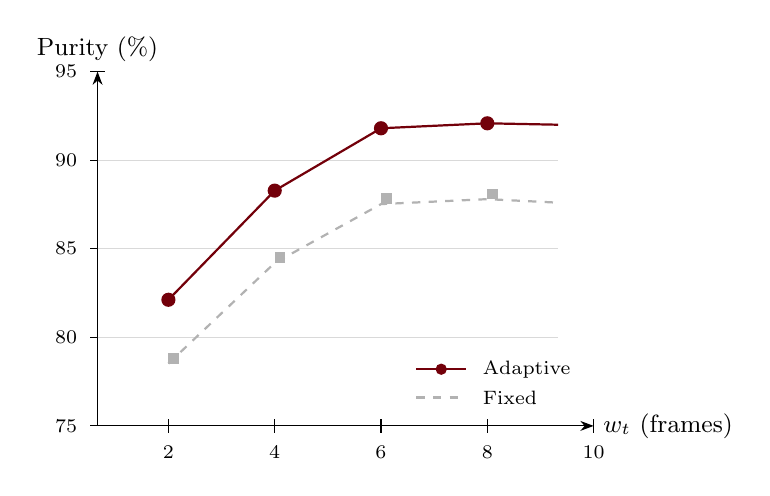
\begin{tikzpicture}[scale=0.9]
    % Axes
    \draw[-{Stealth}, black] (0,0) -- (7,0) node[right, font=\small] {$w_t$ (frames)};
    \draw[-{Stealth}, black] (0,0) -- (0,5) node[above, font=\small] {Purity (\%)};
    
    % Y-axis labels
    \foreach \y/\label in {0/75, 1.25/80, 2.5/85, 3.75/90, 5/95} {
        \draw[black] (-0.1,\y) -- (0.1,\y);
        \node[left, font=\scriptsize] at (-0.15,\y) {\label};
    }
    
    % X-axis labels
    \foreach \x/\label in {1/2, 2.5/4, 4/6, 5.5/8, 7/10} {
        \draw[black] (\x,-0.1) -- (\x,0.1);
        \node[below, font=\scriptsize] at (\x,-0.15) {\label};
    }
    
    % Grid
    \draw[gray!30] (0,1.25) -- (6.5,1.25);
    \draw[gray!30] (0,2.5) -- (6.5,2.5);
    \draw[gray!30] (0,3.75) -- (6.5,3.75);
    
    % Adaptive curve (garnet)
    \draw[garnet, thick] 
        (1,1.78) -- (2.5,3.32) -- (4,4.2) -- (5.5,4.27) -- (6.5,4.25);
    \foreach \x/\y in {1/1.78, 2.5/3.32, 4/4.2, 5.5/4.27} {
        \fill[garnet] (\x,\y) circle (0.1);
    }
    
    % Fixed curve (gray dashed)
    \draw[gray!60, thick, dashed] 
        (1,0.88) -- (2.5,2.3) -- (4,3.13) -- (5.5,3.2) -- (6.5,3.15);
    \foreach \x/\y in {1/0.88, 2.5/2.3, 4/3.13, 5.5/3.2} {
        \fill[gray!60] (\x,\y) rectangle ++(0.15,0.15);
    }
    
    % Legend
    \draw[garnet, thick] (4.5,0.8) -- (5.2,0.8);
    \fill[garnet] (4.85,0.8) circle (0.08);
    \node[right, font=\scriptsize] at (5.3,0.8) {Adaptive};
    
    \draw[gray!60, thick, dashed] (4.5,0.4) -- (5.2,0.4);
    \node[right, font=\scriptsize] at (5.3,0.4) {Fixed};
\end{tikzpicture}
\end{document}
